\chapter{数字电路}\label{chap7}
泰拉瑞亚中有逻辑门,自然也就会有数字电路理论。又因为游戏特性,泰拉瑞亚中的数字电路体系与现实生活中的几乎完全不同。所以不要抱有以下两种幻想:
\begin{itemize}
    \item 我在现实中学过(数字)电路,所以我也能轻松搞定泰拉瑞亚电路。
    \item 我泰拉瑞亚电路很熟,所以我也一定能搞懂现实中的(数字)电路。
\end{itemize}

本章内容,一是建立泰拉瑞亚中的数字电路体系,二是利用数字电路知识进行电路的极限优化。本章专业性较强,建议有能力的人阅读。

\section{组合逻辑与时序逻辑}
泰拉瑞亚中一共有三种功能不同的逻辑门:与门、异或门和故障逻辑门。电路中的信号传递方式也分为两种:状态传递和激活传递。状态传递是指,如果在一根线上放一个火把,那么火把亮表示这根线的状态是1,火把灭表示这根线的状态是0;激活传递是指,在某个特定的逻辑帧,电线激活表示1,不激活表示0。所有电线全部为状态传递的电路称为组合逻辑电路,有至少一根电线为激活传递的电路称为时序逻辑电路。

组合逻辑电路的特点是电路中只有与门和异或门,并且每根线只在某个固定的逻辑帧激活(逻辑延迟器中的爆门除外)。组合逻辑的每个输出都对应一个真值表。

时序逻辑电路利用激活与否来传递信息,同一根电线可能在不同的逻辑帧激活,并且不同逻辑帧激活可能表示不同的信号。递次电路就是一种典型的纯时序逻辑电路。

与现实的数电不同,泰拉瑞亚中的组合逻辑和时序逻辑没有功能上的明确限制。有很多电路既可以用组合逻辑实现,也可以用时序逻辑实现。组合逻辑电路和时序逻辑电路各有优劣,一个电路选择使用组合还是时序,取决于电路本身的特点。
\begin{itemize}
\item 在组合逻辑电路中,整个电路的运行状态可以直接通过读灯得到,如果出了bug,直接看哪个灯的状态不对,就能找到问题。相比较而言,如果时序逻辑电路出了bug,除非借助MechScope,否则很难进行调试。
\item 由于逻辑灯接线取向的问题,时序逻辑电路中经常要出现违背逻辑灯取向的反向绕线,接线比组合逻辑更困难。
\item 为了逻辑同步,复杂的电路中经常会用到逻辑延迟器。组合逻辑电路中每个数据都需要设计一个独立的逻辑延迟器,而时序逻辑电路中可以让所有数据共享一个逻辑延迟器。将所有待传输的数据暂时存储起来,然后由中央逻辑延迟器发送信号释放这个数据。这一点现在很难看明白,后面在除法器部分会体现的很清楚。
\end{itemize}

很多电路概念都分为状态和激活两种情况,也可以分别归类为组合逻辑和时序逻辑。例如加重压力板属于组合逻辑电源,而普通压力板属于时序逻辑电源;火把属于组合逻辑用电器,而像素盒属于时序逻辑用电器。

组合逻辑电路的设计需要用到布尔代数知识。

\section{布尔代数}

\subsection{布尔运算}\label{sec23}
一个数为\textbf{布尔值},是指这个数的取值只能为0和1。\textbf{布尔运算}是对布尔值进行的运算。我们把表达式中的布尔值与布尔常数1简称为\textbf{字母}。

泰拉瑞亚中一共有四种初等布尔运算,它们的运算规则如下,在电路中的意义见\autoref{fig1}:
\paragraph*{取反}$\textrm{\~{}} 0=1,\textrm{\~{}} 1=0$
\paragraph*{连接}$00=0,01=1,10=1,11=0$
\paragraph*{与}$0\&0=0,0\&1=0,1\&0=0,1\&1=1$
\paragraph*{异或}$\textrm{\^{}}(a_1,a_2,\cdots,a_n)=\left\{\begin{array}{ll}1 & \textrm{如果}a_1,\cdots,a_n\textrm{中恰好有一个为}1 \\0&\textrm{其他情况}\end{array}\right.$

\begin{figure}[!ht]
    \centering
    \subfloat[取反:$A=\textrm{\~{}}B$, $B=\textrm{\~{}}A$]{
\includegraphics{images/348.png}\qquad
\includegraphics{images/349.png}}\\
    \subfloat[连接:$B=AC$]{
\includegraphics{images/350.png}\qquad
\includegraphics{images/351.png}}\\
    \subfloat[与:$C=A\&B$]{
\includegraphics{images/352.png}\qquad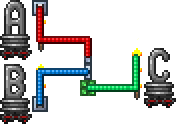
\includegraphics{images/353.png}}\\
    \subfloat[异或:$D=\textrm{\^{}}(A,B,C)$]{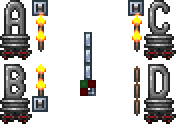
\includegraphics{images/354.png}\qquad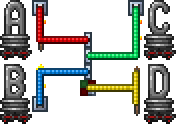
\includegraphics{images/355.png}}
    \caption{初等布尔运算对应的电路。注意取反运算和连接运算不需要逻辑门。}
    \label{fig1}
\end{figure}

此外,在进行分析的时候,为了便于理解,我们也使用其他一些布尔运算,它们都可以由初等布尔运算导出。\autoref{fig2}展示了使用与运算导出或运算的方法。\autoref{tab2}展示了常用的非初等布尔运算。

\begin{figure}[!ht]
    \centering
	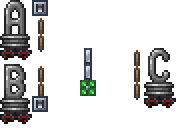
\includegraphics{images/356.png}\qquad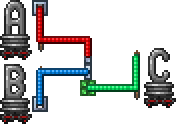
\includegraphics{images/357.png}
    \caption{与运算导出的或运算。$C=A|B$}
    \label{fig2}
\end{figure}

\begin{table}[!ht]
\centering
\begin{tabular}{|c|c|c|}
\hline
运算名称&记号&导出公式\\\hline
或&$a|b$&$\textrm{\~{}}(\textrm{\~{}}a\&\textrm{\~{}}b)$\\\hline
小于&$a<b$&$\textrm{\~{}}a\&b$\\\hline
大于&$a>b$&$a\&\textrm{\~{}}b$\\\hline
等于&$a==b$&$\textrm{\~{}}ab$\\\hline
小于等于&$a\le b$&$\textrm{\~{}}(a\&\textrm{\~{}}b)$\\\hline
大于等于&$a\ge b$&$\textrm{\~{}}(\textrm{\~{}}a\&b)$\\\hline
不等于&$a!=b$&$ab$\\\hline
\end{tabular}
\caption{常用的非初等布尔运算。}\label{tab2}
\end{table}

\subsection{初等布尔运算的性质}\label{sec9317}

\paragraph*{交换律、分配律、结合律}

连接、与、异或都满足\textbf{交换律},改变这些运算下的字母顺序,结果不变。连接、与都满足\textbf{结合律},但是异或不满足结合律,因为$1=\textrm{\^{}}(\textrm{\^{}}(1,1),1)\ne \textrm{\^{}}(1,1,1)=0$。当$a\&b=0$时(这个条件必不可少!),与和连接满足\textbf{分配律}$ab\&c=(a\&c)(b\&c)$。

\paragraph*{其他常用运算律}
\begin{center}
\begin{tabular}{|c|c|c|c|}
\hline
&连接&与&异或\\\hline
与0的运算&$0a=a$&$0\&a=0$&$\textrm{\^{}}(0,a_1,\cdots,a_n)=\textrm{\^{}}(a_1,\cdots,a_n)$\\\hline
与1的运算&$1a=\textrm{\~{}} a$&$1\&a=a$&$\textrm{\^{}}(1,a_1,\cdots,a_n)=\textrm{\~{}} a_1\&\cdots\&\textrm{\~{}} a_n$\\\hline
与自身的运算&$aa=0$&$\begin{aligned}a\& a&=a\\\textrm{\~{}} a\& a&=0\end{aligned}$&\\\hline
转化运算&$\textrm{\^{}}(a,b)=ab$&$a\&b=\textrm{\~{}} ab\&b$&$\begin{aligned}[]&\textrm{\^{}}(a_1,a_2,a_3,\cdots,a_n)=\\&\textrm{\^{}}(\textrm{\~{}} a_1a_3\cdots a_n,\textrm{\~{}} a_2a_3\cdots a_n,a_3,\cdots,a_n)\end{aligned}$\\\hline
\end{tabular}
\end{center}

这里我们证明一下异或的转化运算。
\begin{proof}
令$b=a_1a_2\cdots a_n$,则$a_1a_3\cdots a_n=ba_2$,$a_2a_3\cdots a_n=ba_1$。

假设$\textrm{\^{}}(a_1,a_2,a_3,\cdots,a_n)=1$,那么$a_1,\cdots,a_n$中有且只有1个1,所以$b=1$。从而
\[\begin{split}
&\textrm{\^{}}(\textrm{\~{}} a_1a_3\cdots a_n,\textrm{\~{}} a_2a_3\cdots a_n,a_3,\cdots,a_n)\\
=&\textrm{\^{}}(\textrm{\~{}}ba_2,\textrm{\~{}}ba_1,a_3,\cdots,a_n)\\
=&\textrm{\^{}}(a_1,a_2,a_3,\cdots,a_n)=1.
\end{split}\]

反过来,假设$\textrm{\^{}}(\textrm{\~{}} a_1a_3\cdots a_n,\textrm{\~{}} a_2a_3\cdots a_n,a_3,\cdots,a_n)=1$。令$b_1=\textrm{\~{}} a_1a_3\cdots a_n$,$b_2=\textrm{\~{}} a_2a_3\cdots a_n$,则$\textrm{\^{}}(b_1,b_2,a_3,\cdots,a_n)=1$。与前面同理可推出$\textrm{\^{}}(\textrm{\~{}} b_1a_3\cdots a_n,\textrm{\~{}} b_2a_3\cdots a_n,a_3,\cdots,a_n)=1$。简单计算可知$\textrm{\~{}} b_1a_3\cdots a_n=a_1$,$\textrm{\~{}} b_2a_3\cdots a_n=a_2$,所以$\textrm{\^{}}(a_1,a_2,a_3,\cdots,a_n)=1$。$\hfill\blacksquare$
\end{proof}

\paragraph*{其他记号}
当我们要处理一组布尔值时,我们可以给它们编号。例如一个八位二进制数可以表示为$[a_7,a_6,a_5,a_4,a_3,a_3,a_1,a_0]$,简记为$a_{7:0}$。$a_{7:0}$的最高位是$a_7$,最低位是$a_0$。$a_{7:0}$可以分成两个四位二进制数$a_{3:0}$(可以叫做低四位)和$a_{7:4}$(可以叫做高四位)。

\subsection{真值表}
对于稍微复杂的逻辑表达式,例如$\textrm{\~{}}ab\&\textrm{\~{}}bc\&abc$,我们很难一眼看出它们表达的意义。例子里的表达式只包含三种字母,它们只有8种取值的可能性,所以我们可以直接把这8种情况穷举出来,看看每种情况下这个表达式的结果是什么。

\begin{table}[!ht]
\centering
\begin{tabular}{|c|c|c||c|}
\hline
$a$&$b$&$c$&$\textrm{\~{}}ab\&\textrm{\~{}}bc\&abc$\\\hline
0&0&0&0\\\hline
0&0&1&0\\\hline
0&1&0&0\\\hline
0&1&1&0\\\hline
1&0&0&0\\\hline
1&0&1&0\\\hline
1&1&0&0\\\hline
1&1&1&1\\\hline
\end{tabular}
\caption{$\textrm{\~{}}ab\&\textrm{\~{}}bc\&abc$的真值表。}\label{tab2308}
\end{table}

从\autoref{tab2308}可以看出来,当且仅当$a,b,c$全为1时,$\textrm{\~{}}ab\&\textrm{\~{}}bc\&abc$的值才为1,这不就是与逻辑吗?所以我们得到$\textrm{\~{}}ab\&\textrm{\~{}}bc\&abc=a\&b\&c$,这个逻辑就很好理解了。\autoref{tab2308}就称为$\textrm{\~{}}ab\&\textrm{\~{}}bc\&abc$的\textbf{真值表}。

更多的时候,我们先得到一个真值表,然后希望得出它的逻辑表达式。例如对于显示器而言(\autoref{fig4}),我们在一开始只知道每个显示单元对于哪些输入应该亮,哪些输入应该暗,而不知道应该如何搭建这个逻辑。这里遇到的就是已知真值表,求解逻辑表达式的过程。本小节一开始举的那个例子里,因为真值表比较特殊,我们只通过观察就得到了它的逻辑表达式。对于简单观察得不到逻辑表达式的情况,后续一些小节会给出解决方案。
\begin{figure}[!ht]
\centering
\subfloat[]{\label{tab4}
\begin{tabular}{|c|ccccccc|}
\hline
输入&$A$&$B$&$C$&$D$&$E$&$F$&$G$\\\hline
0&1&1&0&1&1&1&1\\
1&0&0&0&1&0&0&1\\
2&1&0&1&1&1&1&0\\
3&1&0&1&1&0&1&1\\
4&0&1&1&1&0&0&1\\
5&1&1&1&0&0&1&1\\
6&1&1&1&0&1&1&1\\
7&1&0&0&1&0&0&1\\
8&1&1&1&1&1&1&1\\
9&1&1&1&1&0&1&1\\\hline
\end{tabular}}\qquad
\subfloat[]{\raisebox{-80pt}{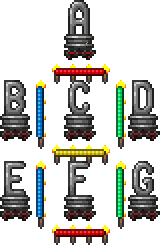
\includegraphics{images/35.png}\label{fig3}}}
\caption{\protect\subref{tab4}十进制数显的真值表;\protect\subref{fig3}七段线接法。}\label{fig4}
\end{figure}

\subsection{字符串的线性相关与秩}
回顾我们把逻辑表达式中的布尔值与布尔常数1简称为字母。我们把由若干字母\textbf{连接}而成的表达式称为\textbf{字符串},简称\textbf{串}。由0个字母连接成的表达式记作0,称为\textbf{空串}。0和1两个串称为\textbf{平凡串}。如果两个串恒等,那么这两个串\textbf{相同}。

注意到由连接的性质$1a=\textrm{\~{}} a$,布尔常数1在这个串里起到的作用是取反。例如,由1,a,b组成的不同串有8个\footnote{由n个字母组成的不同的串有多少个?}:0,1,a,b,ab,\~{}a,\~{}b,\~{}ab。一个串中可以包含重复的字母,但是由于连接的性质$aa=0$和$0a=a$,一对重复的字母可以直接抵消。

给定一组串$s_1,\cdots,s_r$,任选其中若干串(至少一个)做连接运算,得到的串称为这组串的一个\textbf{线性组合}。如果一组非平凡串有一个平凡的线性组合,那么我们称这组非平凡串\textbf{线性相关}。否则,如果一组非平凡串的所有线性组合都是非平凡串,那么我们称这组非平凡串\textbf{线性无关}。一组非平凡串的最大的线性无关子集的大小称为这组非平凡串的\textbf{秩}。
\begin{theorem}{}{thm1}
记一组串的秩为$r$,那么这组串拥有的不同非平凡线性组合数量为$2^r-1$。反之,一组串拥有的不同非平凡线性组合数量一定有形式$2^r-1$,并且在该形式下这组串的秩为$r$。
\end{theorem}
\begin{corollary}{}{thm2}
秩为$r$的一组互不相同的非平凡串至多有$2^r-1$个。$n$个互不相同的非平凡串的秩至少为$\lceil\log_2 (n+1)\rceil$。
\end{corollary}

\begin{example}
考虑三个串$ab$,$abc$,$abcd$。

令$A=ab,B=abc,C=abcd$,那么$A,B,C$的所有不同线性组合为$A=ab,B=abc,C=abcd,AB=c,AC=cd,BC=d,ABC=abd$。所有线性组合都是非平凡串,所以ab,abc,abcd线性无关,\{ab,abc,abcd\}的最大线性无关子集就是它自己,所以ab,abc,abcd的秩是3。
\end{example}

\begin{example}
考虑三个串bc,ac,ab。

令$A=bc,B=ac,C=ab$,那么$A,B,C$的所有不同线性组合为$A=BC=bc,B=AC=ac,C=AB=ab,ABC=0$。$ABC=0$是平凡串,所以bc,ac,ab线性相关。A和B的所有线性组合为$A=bc,B=ac,AB=ab$,都是非平凡串,所以bc,ac线性无关,所以bc,ac,ab的秩为2。
\end{example}

\subsection{简单逻辑及其复杂度}
\textbf{简单逻辑}指只用一个与门或异或门就可以实现的逻辑。这个概念很好理解,但是其复杂度比我们想象的大得多。

考虑一个简单的例子。假设我们现在用一个两灯与门做出了$a\&b$的逻辑,在游戏中,我们要用两种不同颜色的线分别连接到两个逻辑灯。实际应用中有时出于接线考虑,可以利用与逻辑的交换律将$a$与$b$换位。但是等价的逻辑还远不止这两个。在\autoref{sec9317}的转化运算中,看到$a\&b=\textrm{\~{}} ab\&b$,同理$a\&b=\textrm{\~{}} ab\&a$,再利用交换律,又有$a\&b=b\&\textrm{\~{}} ab=a\&\textrm{\~{}} ab$。因此,$a\&b$的等价两灯简单逻辑一共有6个,不考虑交换律则有3个。这些等价逻辑每个都代表不同的接线方法,而多样的接线方法可以帮助我们在一些狭小空间内摆线。

类似的,$a\&b\&c$的等价三灯简单逻辑有168个,不考虑交换律则有28个。对于异或逻辑,用转化运算中的另一个公式也可以得到其等价逻辑。
每一个逻辑都对应一种接线,这么多种等价逻辑就会带来很多种接线方式,也就会增加我们考虑问题的复杂度。一般情况下这么多种接线方式中总有一些可以满足要求,但是一旦不行,我们就需要引入复杂度还要高得多的单步逻辑。

168种等价逻辑是怎么算出来的呢?如此的工作量对于人工来说,即使再有技巧都是无法接受的,更不提人工可能漏算错算的情况。对于简单逻辑,我们开发了软件TCLC(Terraria Combinational Logic Calculator),你只需要输入这个逻辑的\textbf{真值表},它就会用穷举法找出那些满足要求的逻辑。程序下载\url{https://www.bbstr.net/threads/154/}。这个软件只进行了初步开发,因为目前还没有多少实际需求。如果你有更多的需求或想法,可以联系我。

\subsection{单步逻辑及其复杂度}
\textbf{单步逻辑}是若干简单逻辑连接而成的结果。“单步”的意思是这个逻辑在一个逻辑帧内就可以结算完毕,或者说输入与输出只间隔一个逻辑帧。类似的我们也有$k$步逻辑。

单步逻辑有什么用呢?如果电路中要同时执行多个简单逻辑,可以将其中若干逻辑进行连接以获取可能的简化。这个描述非常抽象,我们来看一个例子。

\begin{figure}[!htp]
\centering
\subfloat[可密堆叠的数显]{\label{fig27}
\makecell{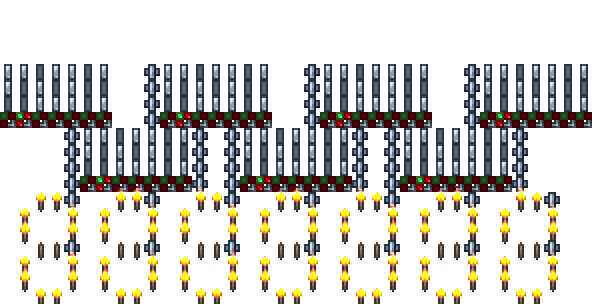
\includegraphics[width=0.99\textwidth]{images/321.png}\\
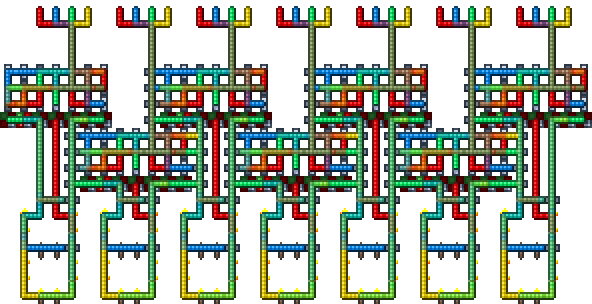
\includegraphics[width=0.99\textwidth]{images/322.png}}}\\
\subfloat[控制部分]{
\includegraphics[width=0.99\textwidth]{images/323.png}}\\
\subfloat[显示部分]{
\includegraphics{images/324.png}}
\caption{}\label{fig26}
\end{figure}

\autoref{fig26}展示了一个BCD数显。这个数显是目前发现的唯一一个可密堆叠(\autoref{fig27})的BCD数显。可密堆叠的要求是极其苛刻的。首先,因为下方显示器的宽度相当小,控制电路的宽度也非常有限;其次,上层和下层控制单元需要可以挨在一起但是线不能连接。这些条件看上去非常不可思议,但是数显能做出来,得益于单步逻辑的超高复杂度。这个数显一共有7个输出,并且因为它们的秩为7,至少需要7个逻辑门。输入接进来时,在逻辑灯上可以有各种接线可能;逻辑门可以选取与和异或,逻辑灯数量也可以改变;输出时,多个逻辑门可以输出到同一根线上实现连接运算;电线在显示器上也可以连接若干段。这么算下来,不考虑正确性的情况下,一个简单数显的接线排列组合可以有成千上万种。从这么复杂的情况中找出一种可行方案不算太困难,但是也需要相当的观察力与经验。

\begin{example}\label{exa3}
某组合逻辑有三个输入$a,b,c$和两个输出$d,e$,其真值表如\autoref{tab13}所示,试设计电路。
\begin{table}[!ht]
\centering
\begin{tabular}{|ccc|cc|c|}
\hline
$a$&$b$&$c$&$d$&$e$&$de$\\\hline
0&0&0&0&0&0\\\hline
0&0&1&0&1&1\\\hline
0&1&0&0&1&1\\\hline
0&1&1&1&0&1\\\hline
1&0&0&0&1&1\\\hline
1&0&1&1&0&1\\\hline
1&1&0&1&0&1\\\hline
1&1&1&1&1&0\\\hline
\end{tabular}
\caption{}\label{tab13}
\end{table}
\end{example}
\begin{proof}[解]
利用TCLC,我们可以算出$d$有四灯表示,$e$有单灯表示:
\begin{align*}
d&=\textnormal{\^{}}(abc,\textnormal{\~{}}c,\textnormal{\~{}}b,\textnormal{\~{}}a)=\textnormal{\~{}}\textnormal{\^{}}(c,b,a,\textnormal{\~{}}abc)\\
e&=abc
\end{align*}
这里$d$和$e$都是用简单逻辑表达的。如果觉得$d$的表达式太复杂\footnote{事实上对于$n$个输入的逻辑,我们的期望是使用$n-1$个灯就能完成,这里的结果显然不尽如人意。},我们可以考虑使用不借助逻辑门的连接运算。

考虑$de$的真值表(\autoref{tab13}的最右边一列),我们可以算出$de$有双灯表示:
$$de=\textnormal{\~{}}ac\&\textnormal{\~{}}ab=\textnormal{\~{}}bc\&\textnormal{\~{}}ab=\textnormal{\~{}}bc\&\textnormal{\~{}}ac$$

\begin{figure}[!ht]
\centering
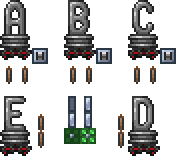
\includegraphics{images/406.png}
\qquad
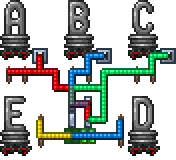
\includegraphics{images/407.png}
\caption{}\label{fig36}
\end{figure}

这样一来,$e$仍用单灯表示,而$d$使用双灯与单灯的连接:$d=dee=(de)e$,我们就得到了\autoref{fig36}所示的电路。在这个例子中,我们通过考虑输出之间的连接减少了灯数。另一方面,考虑连接的逻辑为我们开阔了思路,增加了更多可能性,让我们更有希望设计出满足苛刻条件的电路。
\end{proof}

类似的例子还有使用加三移位法做的二进制与十进制互化的逻辑单元,相关内容会在后面讲到。

\section{算术电路}\label{sec34}

\subsection{加法器(Adder)}
加法器的输入是两个整数,输出是两个输入之和。加法器的解决方案有很多,一个最直接的方法就是串联全加器。

全加器是什么?我们来看二进制加法的竖式计算。计算$a_{7:0}+b_{7:0}$时,首先列出\autoref{tab1406}所示的竖式并且把两个加数填入。然后计算$a_0+b_0$,这个结果可能是$00,01,10$。结果的低位直接就是和的最低位,写在$s_0$的位置。结果的高位是最低位向前的进位,写在$c_1$的位置。然后计算$a_1+b_1+c_1$,把结果的低位填入$s_1$,高位作为进位填入$c_2$,依此类推。这整个加法过程可以用\autoref{fig78}所示的电路模拟,这个电路由八个小模块构成,每个小模块计算$a_i+b_i+c_i$,把结果的低位输出为$s_i$,高位输出到下一个小模块$c_{i+1}$。这每个小模块叫做全加器。

\begin{figure}[!ht]
\centering
\subfloat[加法竖式示意图。一般情况下$c_0=0$]{\label{tab1406}
\begin{tabular}{rccccccccc}
加数1&&$a_7$&$a_6$&$a_5$&$a_4$&$a_3$&$a_2$&$a_1$&$a_0$\\
加数2&&$b_7$&$b_6$&$b_5$&$b_4$&$b_3$&$b_2$&$b_1$&$b_0$\\
进位&&$c_7$&$c_6$&$c_5$&$c_4$&$c_3$&$c_2$&$c_1$&$c_0$\\\hline
和&$s_8$&$s_7$&$s_6$&$s_5$&$s_4$&$s_3$&$s_2$&$s_1$&$s_0$
\end{tabular}
}\\
\subfloat[电路执行加法运算]{\label{fig78}
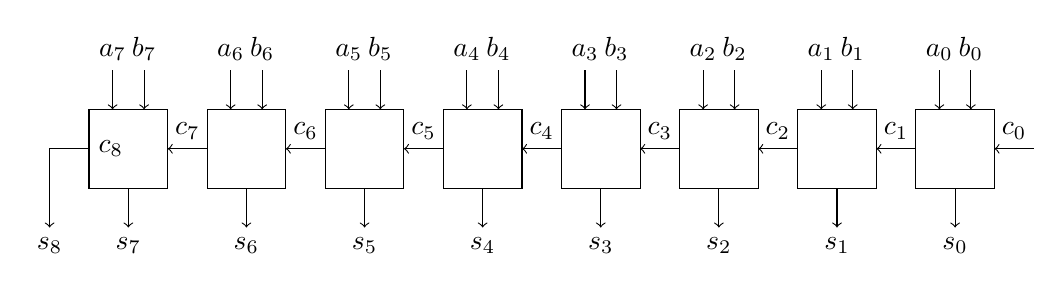
\begin{tikzpicture}[scale=0.5]
    \foreach \x [evaluate={\y=int(7-\x);\z=int(8-\x)}] in {0,1,...,7}
    {
        \draw (3*\x,0) rectangle (3*\x+2,2);
        \draw[->] (3*\x+1,0)  -- (3*\x+1,-1) node[anchor=north] {$s_\y$};
        \draw[->] (3*\x+3,1) -- node[midway,anchor=south] {$c_\y$} (3*\x+2,1);
        \draw[->] (3*\x+0.6,3) node[anchor=south] {$a_\y$} -- (3*\x+0.6,2) ;
        \draw[->] (3*\x+1.4,3) node[anchor=south] {$b_\y$} -- (3*\x+1.4,2) ;
    }
    \draw[->] (0,1) node[anchor=west] {$c_8$} -- (-1,1) -- (-1,-1) node[anchor=north] {$s_8$};
\end{tikzpicture}
}
\caption{}
\end{figure}

全加器接收三个输入$a,b,c_i$,其中$a,b$分别是两个加数,$c_i$是输入进位。全加器产生两个输出$s,c_o$,其中$s$是和,$c_o$是输出进位。全加器的真值表如\autoref{tab1819}。这个逻辑我们在\autoref{exa3}中已经讨论了。

\begin{table}[!ht]
\centering
\begin{tabular}{ccc|cc}
$a$&$b$&$c_i$&$c_o$&$s$\\\hline
0&0&0&0&0\\
0&0&1&0&1\\
0&1&0&0&1\\
0&1&1&1&0\\
1&0&0&0&1\\
1&0&1&1&0\\
1&1&0&1&0\\
1&1&1&1&1
\end{tabular}
\caption{全加器的真值表}\label{tab1819}
\end{table}

\begin{figure}[!ht]
\centering

\includegraphics{images/408.png}
\qquad

\includegraphics{images/409.png}
\caption{四位加法器。红线和蓝线分别表示两个加数,绿线为进位,黄线为和,底端绿线为溢出位。上面低位下面高位。}\label{fig37}
\end{figure}

有了全加器,直接把多个全加器首尾相连,就得到了一个加法器(\autoref{fig37})。这个加法器要求两个加数从低位到高位依次延迟一个逻辑帧输入。

\begin{figure}[!ht]
\centering

\includegraphics{images/410.png}
\qquad

\includegraphics{images/411.png}
\caption{四位累加器。两个加数依次输入红蓝线。上面低位下面高位。}\label{fig38}
\end{figure}

除了用组合逻辑,我们还可以用时序逻辑做加法器。降频电路有逢二进一的特性,所以可以直接用降频电路做一个加法器(\autoref{fig38})。与组合逻辑加法器不同,时序逻辑加法器实质上是累加器,如果不复位,那么每次输入都会直接累加到上一次的结果上。在时序逻辑加法器中,第二个加数各位要在同一个逻辑帧输入,或者低位延迟输入,这与组合逻辑加法器恰好相反。

在加法器上,时序逻辑的另一个优点是,把降频电路改成递次电路,就可以直接做任何进制的累加。\url{https://www.bilibili.com/video/av40474377/}中的进制转换实际上就是做了一个十进制累加器,每修改一个二进制数位就向累加器中加一个值或减一个值。

\subsection{减法器(Subtractor)}
有了补码这个工具,减法器和加法器就可以共用一个电路,我们只需要增加一些部件将其中一个加数取反加一。取反的操作是容易的,而加一的操作正好可以借用\autoref{tab1406}中我们没有用到的$c_0$。做出的组合逻辑加减法器如\autoref{fig39}所示,需要注意的是加法器的输入从低位到高位延迟一个逻辑帧,所以对每个数位取反的时候也要从低位到高位延迟一个逻辑帧,完成这项工作的是\autoref{fig39}中最右边一列逻辑门。

\begin{figure}[!ht]
\centering

\includegraphics{images/412.png}
\qquad

\includegraphics{images/413.png}
\caption{四位加减法器。顶端黄线控制加减法,0为加法,1为减法。计算加法时红线和蓝线分别表示两个加数。计算减法时蓝线为被减数,红线为减数。黄线为和,底端绿线为溢出位。上面低位下面高位。}\label{fig39}
\end{figure}

时序逻辑的减法器同样是使用补码运算,这里不给出具体实现。

\subsection{比较器(Comparator)}
比较两个数的大小,最简单的就是从高位向低位逐位比较。例如比较$a_{[7:0]}$和$b_{[7:0]}$两个8位二进制数,首先比较最高位$a_7$和$b_7$,如果它们相等再比较$a_6$和$b_6$,依此类推。最后我们可以得到一个逻辑表达式:
\[\begin{split}
a_{[7:0]}\mathtt{>}b_{[7:0]}=&(a_7\mathtt{>}b_7)(a_7\mathtt{==}b_7\& a_6\mathtt{>}b_6)(a_7\mathtt{==}b_7\& a_6\mathtt{==}b_6\& a_5\mathtt{>}b_5)\\
&(a_7\mathtt{==}b_7\& a_6\mathtt{==}b_6\& a_5\mathtt{==}b_5\& a_4\mathtt{>}b_4)\\
&(a_7\mathtt{==}b_7\& a_6\mathtt{==}b_6\& a_5\mathtt{==}b_5\& a_4\mathtt{==}b_4\& a_3\mathtt{>}b_3)\\
&(a_7\mathtt{==}b_7\& a_6\mathtt{==}b_6\& a_5\mathtt{==}b_5\& a_4\mathtt{==}b_4\& a_3\mathtt{==}b_3\& a_2\mathtt{>}b_2)\\
&(a_7\mathtt{==}b_7\& a_6\mathtt{==}b_6\& a_5\mathtt{==}b_5\& a_4\mathtt{==}b_4\& a_3\mathtt{==}b_3\& a_2\mathtt{==}b_2\& a_1\mathtt{>}b_1)\\
&(a_7\mathtt{==}b_7\& a_6\mathtt{==}b_6\& a_5\mathtt{==}b_5\& a_4\mathtt{==}b_4\& a_3\mathtt{==}b_3\& a_2\mathtt{==}b_2\& a_1\mathtt{==}b_1\& a_0\mathtt{>}b_0)
\end{split}\]
用\autoref{sec23}中的导出公式,我们得到了只包含初等布尔运算的逻辑表达式:
\[\begin{split}
a_{[7:0]}>b_{[7:0]}=&(a_7\&\textrm{\~{}}b_7)(\textrm{\~{}}a_7b_7\& a_6\&\textrm{\~{}}b_6)(\textrm{\~{}}a_7b_7\&\textrm{\~{}}a_6b_6\& a_5\&\textrm{\~{}}b_5)\\
					&(\textrm{\~{}}a_7b_7\&\textrm{\~{}}a_6b_6\&\textrm{\~{}}a_5b_5\& a_4\&\textrm{\~{}}b_4)\\
					&(\textrm{\~{}}a_7b_7\&\textrm{\~{}}a_6b_6\&\textrm{\~{}}a_5b_5\&\textrm{\~{}}a_4b_4\& a_3\&\textrm{\~{}}b_3)\\
					&(\textrm{\~{}}a_7b_7\&\textrm{\~{}}a_6b_6\&\textrm{\~{}}a_5b_5\&\textrm{\~{}}a_4b_4\&\textrm{\~{}}a_3b_3\& a_2\&\textrm{\~{}}b_2)\\
					&(\textrm{\~{}}a_7b_7\&\textrm{\~{}}a_6b_6\&\textrm{\~{}}a_5b_5\&\textrm{\~{}}a_4b_4\&\textrm{\~{}}a_3b_3\&\textrm{\~{}}a_2b_2\& a_1\&\textrm{\~{}}b_1)\\
					&(\textrm{\~{}}a_7b_7\&\textrm{\~{}}a_6b_6\&\textrm{\~{}}a_5b_5\&\textrm{\~{}}a_4b_4\&\textrm{\~{}}a_3b_3\&\textrm{\~{}}a_2b_2\&\textrm{\~{}}a_1b_1\& a_0\&\textrm{\~{}}b_0)
\end{split}\]

\begin{figure}
\centering
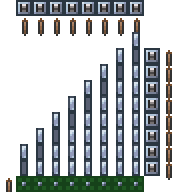
\includegraphics{images/396.png}\qquad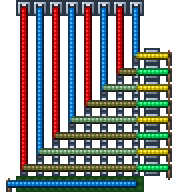
\includegraphics{images/397.png}
\caption{逐位比较器。上方火把表示$b_{[7:0]}$,左边高位右边低位;右侧火把表示$a_{[7:0]}$,下方高位上方低位;左下火把表示$a_{[7:0]}\mathtt{>}b_{[7:0]}$。}\label{fig33}
\end{figure}
将这个逻辑表达式转换为电路如\autoref{fig33}所示。

比较两个数的大小,除了逐位比较之外,还可以直接将两个数做减法,并判断结果的正负性。减法器我们已经做过了,而补码表示中,一个数的正负可以直接通过最高位得出。这里有两个细节的问题。无符号整数没有符号位,如何比较两个无符号整数的大小?有符号整数的两数之差可以达到$127-(-128)=255=11111111$,而这个数作为有符号整数实际上表示$-1$,即小于0。如何处理这些特殊情况?事实上我们这里的比较器只能比较无符号整数,而所谓的“最高位”实际上指的是\autoref{tab1406}中的溢出位$s_8$。对于有符号整数有两种处理方法:第一种是首先判断符号,如果符号相等,再做无符号整数的比较;第二种是把两个数都加$128$,这样就把$-128\sim127$的范围变成了$0\sim255$,然后做无符号整数的比较即可。

比较两个数是否相等,也有两种解法,一种是直接逐位比较,另一种是判断它们的差是否为0。这两种方法并没有绝对的优劣,虽然逐位比较的电路会比较简单,但是判断差值的电路可以直接附加在其他功能上,例如加法器。

\subsection{乘法器(Multiplier)}
乘法是加法的推广,乘法器也是加法器的推广。我们首先来看二进制乘法的竖式计算。因为乘法规模较大,这里给出4位乘法的例子(\autoref{tab6585})。

\begin{figure}[!ht]
$$
\begin{array}{ccccccccc}
&&&&a_3&a_2&a_1&a_0\\
&&&&b_3&b_2&b_1&b_0\\\hline
&&&&b_0\&a_3&b_0\&a_2&b_0\&a_1&b_0\&a_0\\
&&&b_1\&a_3&b_1\&a_2&b_1\&a_1&b_1\&a_0\\
&&b_2\&a_3&b_2\&a_2&b_2\&a_1&b_2\&a_0\\
&b_3\&a_3&b_3\&a_2&b_3\&a_1&b_3\&a_0\\\hline
H_3&H_2&H_1&H_0&l_3&l_2&l_1&l_0
\end{array}
$$
\caption{乘法竖式计算}\label{tab6585}
\end{figure}

从\autoref{tab6585}可以看出来,做一个4位乘法实际上就是做4个数的加法。4个数的加法,可以按照运算顺序拆分成三次2个数的加法,如\autoref{fig79}所示。

\begin{figure}[!ht]
\centering
\begin{tikzpicture}
    \draw (0,0) rectangle node{加法器} (5,1);
    \draw (0,2) rectangle node{加法器} (5,3);
    \draw (0,4) rectangle node{加法器} (5,5);
    
    \draw[->] (2,6) node[anchor=south]{$a_1$} -- (2,5);
    \draw[->] (3,6) node[anchor=south]{$a_2$} -- (3,5);
    \draw[->] (2,4)  -- node[midway,anchor=east]{$a_1+a_2$} (2,3);
    \draw[->] (6,3.5) node[anchor=west]{$a_3$} -- (3,3.5) -- (3,3);
    \draw[->] (2,2)  -- node[midway,anchor=east]{$a_1+a_2+a_3$} (2,1);
    \draw[->] (6,1.5) node[anchor=west]{$a_4$} -- (3,1.5) -- (3,1);
    \draw[->] (2.5,0) -- (2.5,-1) node[anchor=north]{$a_1+a_2+a_3+a_4$};
\end{tikzpicture}
\caption{四个加数$a_1,a_2,a_3,a_4$连加}\label{fig79}
\end{figure}

把\autoref{fig79}中的加法器展开成串联的全加器,就得到了四位乘法器的结构示意图(\autoref{fig80})。

\begin{figure}[!ht]
\centering
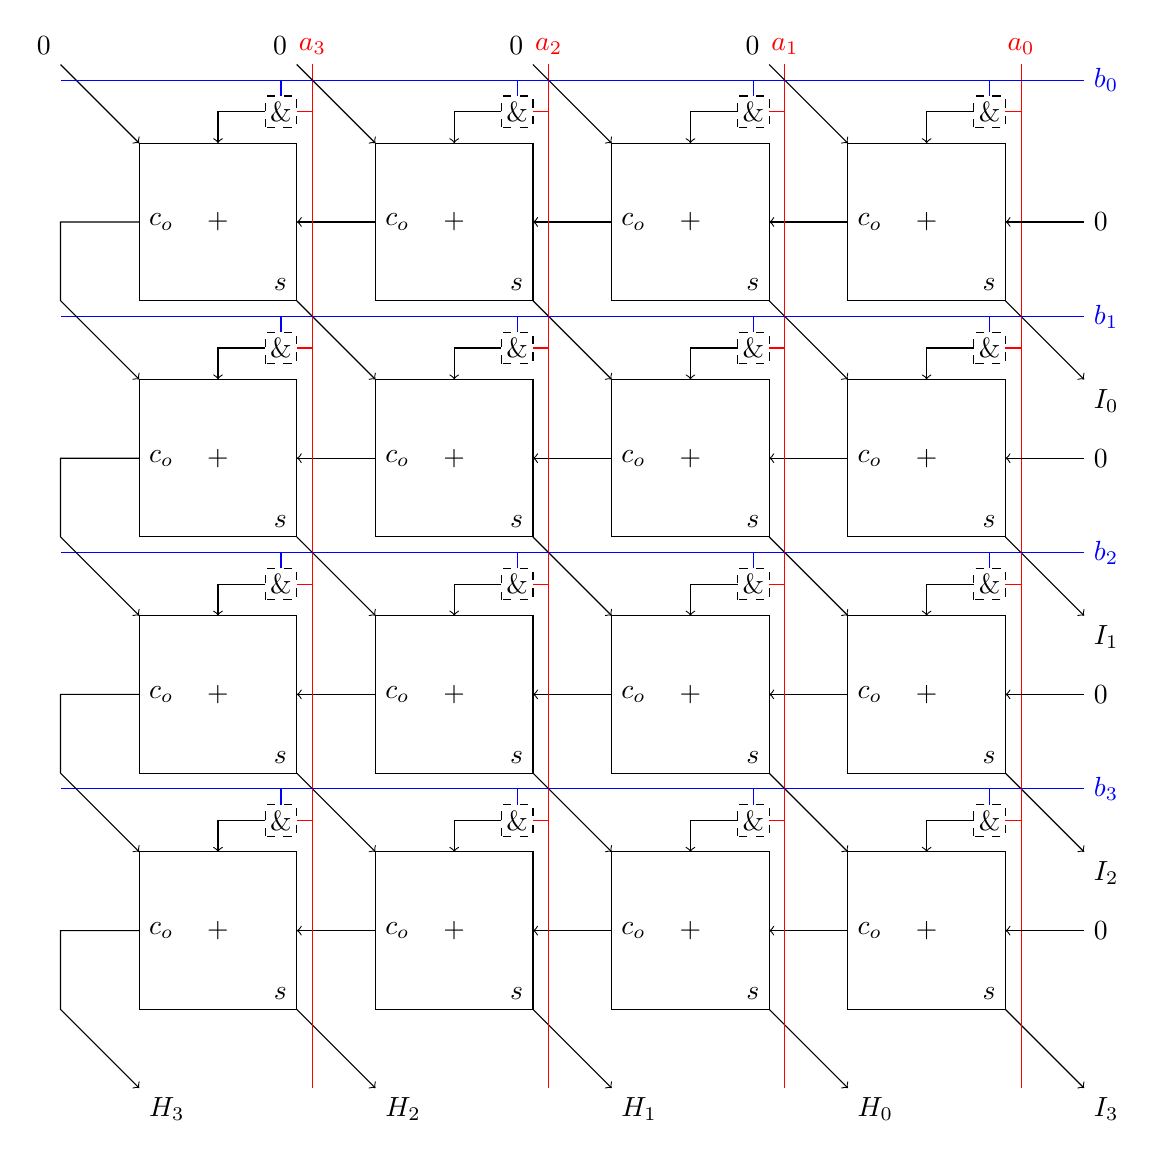
\begin{tikzpicture}
    \foreach \x [evaluate={\z=int(3-\x)}] in {0,1,2,3}
        \foreach \y [evaluate={\w=int(3-\y)}] in {0,1,2,3} {
            \draw (3*\x,3*\y) rectangle node {$+$} (3*\x+2,3*\y+2); % 全加器框架
            \draw[dashed] (3*\x+1.6,3*\y+2.2) rectangle node {\&} (3*\x+2,3*\y+2.6);
            \draw[->] (3*\x+1.6,3*\y+2.4) -- (3*\x+1,3*\y+2.4) -- (3*\x+1,3*\y+2);
            \draw[blue] (3*\x+1.8,3*\y+2.6) -- (3*\x+1.8,3*\y+2.8);
            \draw[red] (3*\x+2,3*\y+2.4) -- (3*\x+2.2,3*\y+2.4);
            \draw[->] (3*\x+2,3*\y) node[anchor=south east] {$s$} -- (3*\x+3,3*\y-1); % 和输出
        }
    \foreach \x in {1,2,3}
        \foreach \y in {0,1,2,3}
            \draw[->] (3*\x,3*\y+1) node[anchor=west] {$c_o$} -- (3*\x-1,3*\y+1); % 进位连接
    \foreach \x [evaluate={\z=int(3-\x)}] in {0,1,2,3}{
        \draw[->,] (3*\x-1,12) node[anchor=south east] {$0$} -- (3*\x,11); % 第一排缺省加数
        \draw (3*\x,-1) node[anchor=north west] {$H_\z$}; % 结果高四位
        \draw[red] (3*\x+2.2,12) node[anchor=south] {$a_\z$} -- (3*\x+2.2,-1); %乘数1输入
    }
    \foreach \y [evaluate={\w=int(3-\y)}] in {0,1,2,3}{
        \draw (12,3*\y-1) node[anchor=north west] {$I_\w$}; % 结果低四位
        \draw[->] (0,3*\y+1) node[anchor=west] {$c_o$} -- (-1,3*\y+1) -- (-1,3*\y) -- (0,3*\y-1); % 左边一列进位输出
        \draw[->] (12,3*\y+1) node[anchor=west] {$0$} -- (11,3*\y+1); % 右边一列进位输入
        \draw[blue] (12,3*\y+2.8) node[anchor=west] {$b_\w$}-- (-1,3*\y+2.8); % 乘数2输入
    }
\end{tikzpicture}
\caption{四位乘法器结构示意图。大的实线方框表示全加器,$c_o$表示进位输出,$s$表示和输出。小的虚线方框表示与门,红蓝线输入,黑线输出。两个乘数分别从上方和右方输入,乘积的低位从右边输出,高位从下边输出。全加器缺少的输入补零。左右相邻的两个全加器,右边的早一个逻辑帧;上下相邻的两个全加器,上边的早两个逻辑帧。}\label{fig80}
\end{figure}

乘法器的单个单元电路见\autoref{fig81},其中用不同颜色的背景墙标记区域和线路。橙色区域为全加器。黄色区域是与门。蓝色线路是从右边输入的乘数,每经过一个单元要延迟1个逻辑帧。红色线路是从上边输入的乘数,每经过一个单元要延迟2个逻辑帧。紫色线路是横向的进位传递。绿色线路是从左上到右下的和传递。

\begin{figure}[!ht]
\centering
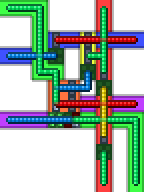
\includegraphics{images/436.png}
\caption{乘法器单个单元的结构}\label{fig81}
\end{figure}

单元堆叠后的效果见\autoref{fig82},其中每个单元大小3*7。优化过程用到了如下的接线技巧:
\begin{itemize}
	\item 左右方向上红蓝线循环,便于接线。
	\item 相邻两列错位,便于进位和横向乘数的传递。
	\item 纵向的逻辑延迟用到了一个异或门,从而这个门不需要为经过的绿线让路。
	\item 与门利用了等式$a\&b=\textrm{\~{}} ab\&b$,便于接线。
\end{itemize}

\begin{figure}[!ht]
\centering
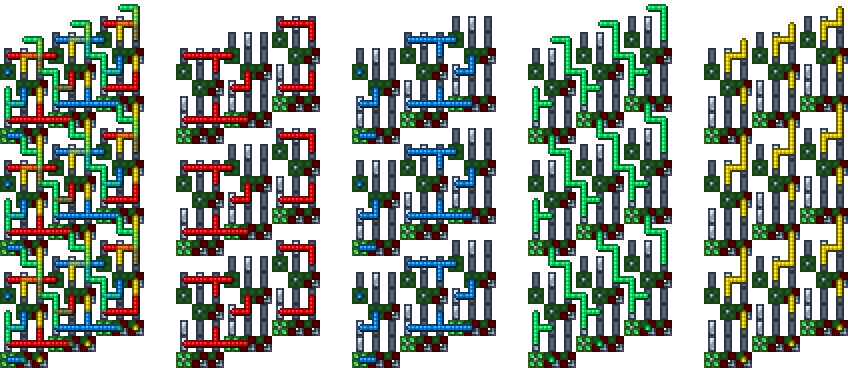
\includegraphics[width=\textwidth]{images/437.png}
\caption{堆叠优化后的效果}\label{fig82}
\end{figure}

\subsection{除法器(Divider)}
1
\subsection{移位器(Shifter)}
移位又分为逻辑移位、算术移位、循环移位,其中逻辑移位和算术移位应用较广。

\begin{figure}[!ht]
\centering
\subfloat[逻辑右移一位]{
\includegraphics{images/414.png}}
\qquad
\subfloat[算术右移一位]{
\includegraphics{images/415.png}}
\qquad
\subfloat[循环右移一位]{
\includegraphics{images/416.png}}
\caption{递次电路移位}\label{fig40}
\end{figure}

如果只移一位的话,这三种移位都可以通过递次电路实现,如\autoref{fig40}所示。

\begin{figure}
\centering
\subfloat[逻辑右移]{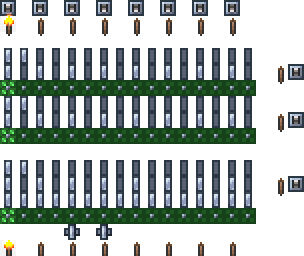
\includegraphics[width=0.45\textwidth]{images/400.png}\qquad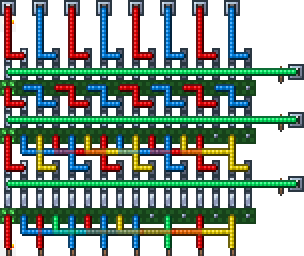
\includegraphics[width=0.45\textwidth]{images/401.png}}

\subfloat[算术右移]{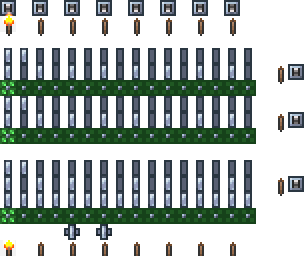
\includegraphics[width=0.45\textwidth]{images/402.png}\qquad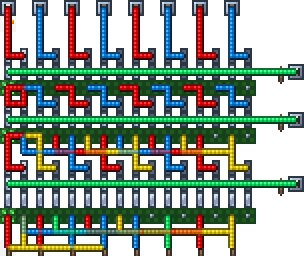
\includegraphics[width=0.45\textwidth]{images/403.png}}

\subfloat[经过简单优化的算术右移]{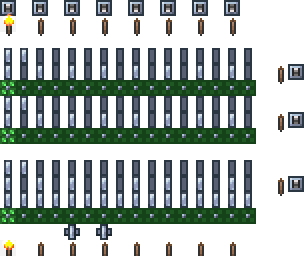
\includegraphics[width=0.45\textwidth]{images/404.png}\qquad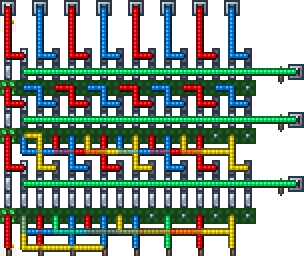
\includegraphics[width=0.45\textwidth]{images/405.png}}
\caption{组合逻辑原理的移位器。右侧三个火把从上到下作用依次为移1位、移2位、移4位。}\label{fig35}
\end{figure}

如果要移任意位,递次电路大概率会爆门,此时需要考虑其他方案。一个简单的思路是使用\autoref{fig35}所示的组合逻辑。这个组合逻辑的缺点是,被移位数的所有数位输入要在同一个逻辑帧,而移位量的数位要在各个逻辑帧依次输入,调节逻辑同步较复杂。此外,由于逻辑门的取向问题,这种方法不适用于循环移位。

\begin{figure}[!ht]
\centering
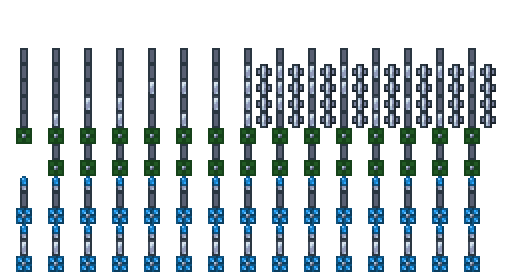
\includegraphics{images/417.png}
\qquad
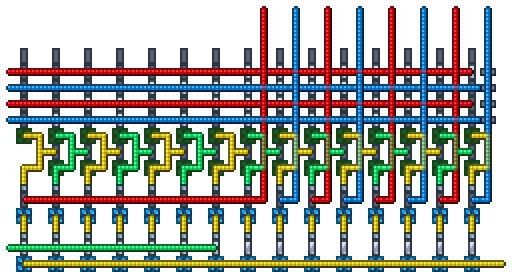
\includegraphics{images/418.png}
\caption{移位器。纵向的红蓝线输入待移位的数。横向红蓝线输入移位的位数。通过顶端的逻辑灯激活对应的输出。底端绿线用于切换逻辑移位和算术移位。}\label{fig41}
\end{figure}

事实上,因为数字电路结构都相对复杂,在泰拉瑞亚中想做一定规模的数字电路,一定要考虑利用\nameref{sec17}技术传输数据。\nameref{sec17}技术通过在不同逻辑帧发送不同数位传播数据,我们可以通过这一特点设计专门兼容\nameref{sec17}的移位器。\autoref{fig41}通过选取网线输出的起始数位实现移位功能。

\subsection{随机数生成器(Random Number Generator)}
在现实中需要用复杂算法实现的功能,在泰拉瑞亚中反而异常简单。直接使用8个1/2概率的故障逻辑门,我们就可以随机生成8位二进制数。
\vspace{5cm}

没了。

\subsection{进制转换}

\paragraph*{方法一} 直接用定义式$a_{n:0}=a_n2^n+a_{n-1}2^{n-1}+\cdots+a_02^0$。要利用这个式子将二进制转换为十进制,需要做一个十进制加法器,然后存储2的各次幂的十进制值。\url{https://www.bilibili.com/video/av40474377/}就是用的这种方法。

十进制转二进制可以用同样的原理,做一个二进制加法器,然后存储10的各次幂的二进制值。

\paragraph*{方法二} 利用\autoref{sec30}和\autoref{sec31}介绍的方法。在竖式的每一步中,我们需要做一个查表的操作,然后错一位。这个查表的操作实际上是一个组合逻辑,如\autoref{tab12}所示。

\begin{table}[!ht]
\centering
\begin{tabular}{|c|c|}
\hline
二进制&BCD\\\hline
0000&0000\\\hline
0001&0001\\\hline
0010&0010\\\hline
0011&0011\\\hline
0100&0100\\\hline
0101&1000\\\hline
0110&1001\\\hline
0111&1010\\\hline
1000&1011\\\hline
1001&1100\\\hline
\end{tabular}
\caption{二进制转BCD则从左到右查,BCD转二进制则从右到左查。}\label{tab12}
\end{table}

二进制转BCD和BCD转二进制对应不同的真值表,我们需要分开设计。

\section{存储电路}
一个存储电路总是要有一个用于存放数据的阵列和一个选择数据的多路选择器。

\subsection{多路选择器(Multiplexer)}
多路选择器接收一个二进制地址,激活该地址代表的位置。一个经典的四位多路选择器如\autoref{fig42}所示。

\begin{figure}[!ht]
\centering

\includegraphics{images/419.png}\vspace{16pt}

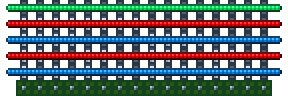
\includegraphics{images/420.png}
\caption{经典四位多路选择器。红蓝线表示地址,上面高位下面低位。绿线双激活输出。16个逻辑门从左到右依次表示0000到1111。}\label{fig42}
\end{figure}

我们在\nameref{sec2:2}中曾见过相似的电路,事实上那个就是状态版的多路选择器。本小节中我们通过\nameref{sec33}实现了激活版的多路选择器。

\subsection{只读存储器(Read-Only Memory)}
只读存储器用于存储事先设计好的、固定的数据。这些数据不需要在使用时修改,所以一般是通过物理方式直接做在电路中。
\begin{figure}[!ht]
    \centering
	\subfloat[横向输入纵向输出]{\label{fig49}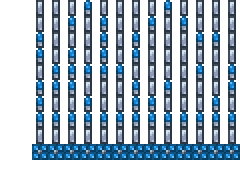
\includegraphics{images/342.png}\quad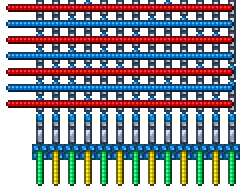
\includegraphics{images/341.png}}
    \qquad
	\subfloat[纵向输入横向输出]{\label{fig50}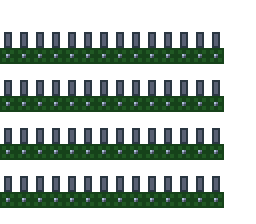
\includegraphics{images/343.png}\quad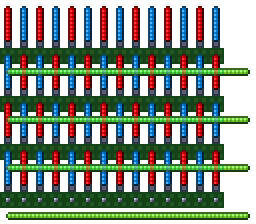
\includegraphics{images/344.png}}
    \qquad
	\subfloat[纵向输入横向输出]{\label{fig51}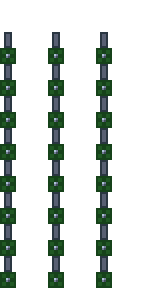
\includegraphics{images/346.png}\quad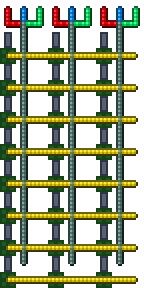
\includegraphics{images/345.png}}
    \caption{ROM的三种设计。}\label{fig48}
\end{figure}
\autoref{fig48}展示了三种ROM设计。\autoref{fig49}使用故障逻辑灯存储数据。一根横线激活时,只有经过的故障逻辑灯下方的逻辑门才会激活。因为存储器要与多路选择器配合,而多路选择器是纵向输出,所以\autoref{fig49}目前没有实用价值。\autoref{fig50}和\autoref{fig51}都是通过接线存储数据,也是有广泛应用的两种ROM。两个电路在实现方式上的区别是,\autoref{fig50}通过连接输出线与逻辑门来存储,而\autoref{fig51}通过连接输入线与逻辑灯来存储。占用空间方面,\autoref{fig50}占用高度较低(1.5格/bit),\autoref{fig51}占用高度较高(2格/bit)。逻辑同步方面,\autoref{fig51}的输出是同步的,而\autoref{fig50}不同步,在本来就需要不同步的场景(例如很多\nameref{sec34}和\nameref{sec17}),\autoref{fig50}更好。

\nameref{sec2:2}中,\autoref{i36:37}就是状态式的多路选择器,\autoref{i42:43}的下半部分电路就是\autoref{fig50}样式的ROM。只有有限个输出情况的显示器都可以通过ROM实现。

\subsection{只写存储器(Write-Only Memory)}
1
\subsection{随机存储器(Random Access Memory)}
1
\subsection{寄存器(Register)}
1
\subsection{栈(Stack)}
1

\section{分段显示器化简理论}
1
\subsection{分段显示器主要结构}
1
\subsection{显示矩阵、分段矩阵和数字矩阵}
1
\subsection{矩阵的初等变换}
1
\subsection{化简原理与细节}
1

\section{处理器结构}
1
\subsection{汇编语言}
1
\subsection{机器语言}
1
\subsection{处理器的拓扑结构}
1
\subsection{数据路径(Data Path)}
1